\documentclass{article}
\usepackage[utf8]{inputenc}
\usepackage{array}
\usepackage{graphicx}
\usepackage{hyperref}
\usepackage{enumitem}
\title{Coding standards}
\author{contrapositives }
\date{May 2019}

\begin{document}
\begin{titlepage}
	\begin{center}
	\huge{University of Pretoria\\
	Software Engineering - COS 301}\\
	\line(1,0){350}\\
	\huge{\bfseries Coding standards document}\\
	\line(1,0){350}\\
	Contrapositives\\
	May 2019\\
	[3cm]
	\end{center}
	\begin{flushleft}
	\bfseries{Authors:}
	\end{flushleft}
	\begin{flushleft}
	Brendan Bath \hspace{32mm}{\textbf{u16023359}}\\
	Musa Mathe			\hspace{34mm}{\textbf{u15048030}}\\
	Jessica da Silva			\hspace{30mm}{\textbf{u16045816}}\\
	Natasha Draper     \hspace{29mm}{\textbf{u16081758}}\\

	\end{flushleft}
\end{titlepage}
\maketitle


\section{BackEnd}
    \subsection{Python}
            \begin{enumerate}
                \item Separate each disjointed statement to be on it's single line.
                \item Use positional system to pass arguments to functions e.g send(message,recipient)
                \item For private properties and implementation details make sure to prefix all "internals" with an underscore.
                \item When a function grows in complexity avoid returning meaningful values from many output points in the body.
                \item If you know the length of a list or tuple, you can assign names to its elements with unpacking e.g for index,item in enumerate(some_list):
                
                \item If you need to assign something (for instance, in Unpacking) but will not need that variable, use underscore
                
                
            \end{enumerate}        
    
\section{FrontEnd}
    \subsection{Vue style}
            
        \begin{enumerate}
            
            \item Add a component on the views sub-directory in the frontend directory
            \item All imports should occur at the top of the page.
            \item Component names should always be meaningful words, e.g Vue.component('Login',{}) , Vue.component('Register',{})
            \item In component \textbf{data} you must not specify the function e.g Vue.component('some-comp', {data:  {return { email: 'email'}}
            \item \textbf{Prop} definitions should be as detailed as possible by atleast specifying types e.g props:{status: String}})
            \item Always use \textbf{key} with v-for e.g \texttt{<ul><li v-for="todo in todos" :key="todo.id" \{{todo.text }\}</li></ul>} in order to maintain internal component state down the subtree.
            \item  Each component should be on its own file to quickly find a component when you need to edit it or review how to use it.
            \item Filenames of single-file components should either be always PascalCase or always kebab-case for autocompletion in code editors, for consistency with how we reference components in JS(X) and templates. e.g MyComponent.vue or my-component.vue
            
            \item Base components that apply app-specific styling and conventions should all begin with a specific prefix, such as App e.g AppFooter
            \item Components with no content should be self-closing in single-file components, string templates but never in DOM templates.
            e.g single-file ,string template \texttt{<MyComponent/> }, DOM template \texttt{<my-component></my-component>}
            
            \item You may want to add one empty line between multi-line properties to avoid components to be cramped and difficult to read.
            
            \item All imports of files should be included at the top of the file.
            
        \end{enumerate}
        
        
\subsection{Typescript}
        \begin{enumerate}
            \item Only single quotes can be used. e.g name:'home'
            \item Use only 2 spaces for indentation.
            \item You can use underscores at the beginning.
            \item Do not use semicolons at the end of every statement e.g
            \item  Arrow functions with one parameter must not have parentheses.
            \item Only use lower CamelCased or UPPER\texttt{_CASED variable names} .
            
        \end{enumerate}
\newpage
\section{General(Style, Structure and layout)}
  
        \subsection{Variables, Methods, Attribute:}
            \begin{enumerate}
                \item Should be short and descriptive.
                \item Should begin with lower case letter.
                \item Upper-case letter should be used immediately after the first name description of the variable.
                \item Should not be a single character e.g. string y
            \end{enumerate}
            
            \subsection{Indendation and layout}
                \begin{enumerate}
                    \item Lines should be kept to a sensible length to make the code easier to read and print.
                    \item Single blank lines should be used to separate methods and to emphasise blocks of code.
                    \item Blocks that are nested more should be indented more.
                \end{enumerate}
            \subsection{Directories}
                \begin{enumerate}
                    \item All tests should be placed in a 'tests' directory.
                    \item All vue components should be placed inside 'view' directory.
                \end{enumerate}
                
            \subsection{Exceptions}
                \begin{enumerate}
                    \item Exceptions should be used where necessary.
                    \item Instead of throwing basic Exception classes, sub-classes should be made with more meaningful names.
                    \item Appropriate catch statements should be put in place to allow the program to recover if need be.
                \end{enumerate}
            \subsection{Commenting}
                \begin{enumerate}
                    \item Use in-line commenting to help the next developer who might be editing your code.
                    \item Inline comments should appear on the line above the code you are commenting.
                    \item Comments should be added within the body of a method if they are used within that method.
                \end{enumerate}
            \subsection{Version control}
                \begin{enumerate}
                    \item No commented out code must be committed unless you have a very good reason that is clearly
described in a comment by the code you are committing.
                \end{enumerate}
                
                \section{Repository}
                    \subsection{Repository definition}
                        \begin{enumerate}
                            \item Do not commit to master branch.
                            \item Do not commit any code with errors , test first to make sure your code is working without breaking any of the main code.
                            \item For each feature you create, create a new feature branch then merge to develop.
                            \item Always create continuous commits as you develop a certain feature.
                            \item All the files should belong to a specific folder.
                            \item Folder names should be descriptive enough to show what they contain.
                        \end{enumerate}
                    \subsection{Repository structure}
                    
\begin{figure}[h]
    \centering
    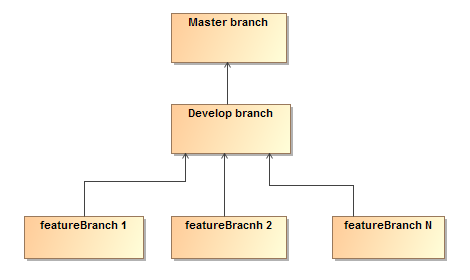
\includegraphics[scale=0.9]{git.PNG}
    \caption{Git structure}
    \label{fig:domain}
\end{figure}

\end{document}
